\section{Overview}

\begin{figure}
    \centering
    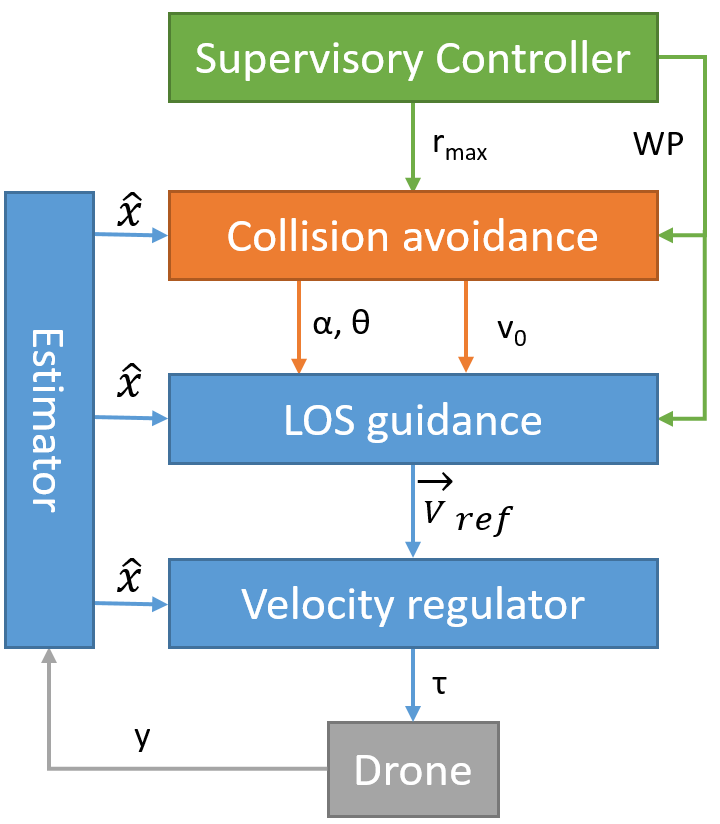
\includegraphics[width = 0.4\textwidth]{Figures/ControlHeirarchy}
    \caption{Control heirarchy. $r_{max}$ is the maximal accepted risk. WP are the waypoints the drone should attempt follow. $\alpha$ and $\theta$ are angle offsets relative the nominal LOS-velocity direction. $v_0$ is the reference speed, $\vec{v}_{ref}$ the reference velocity, $\tau$ are motor torques and forces, $y$ are measurements, and $\hat{x}$ is the estimated state. }
    \label{fig:ControlHeirachy}
\end{figure}

The task is to make a collision avoidance algorithm that works with low resolution radar sensors that incorporates uncertainties in state estimates. To achieve this goal the scenario based model predictive control strategy developed in \cite{Johansen2016} is applied. This strategy simulates different control actions at the initial time point and chooses the best control action based on some objective function. 

The collision avoidance strategy is going to be used in industrial inspection missions. The task of the drone is to follow the straight line between given waypoints, where the drone might have to deviate from the path to avoid collision. The drone is equipped with radar sensors that give a low resolution information about the obstacles. Due to the low resolution, the exact position of obstacles is often unknown. 

The proposed control hierarchy is shown in \ref{fig:ControlHeirachy}. The drone is controlled by a velocity regulator that ensures that the drone moves in the designated direction at the designated speed. This velocity vector is supplied by the line of sight (LOS) guidance law. This guidance law uses the list over waypoints to calculate the velocity reference that gently moves the drone towards and along the correct path. The collision avoidance algorithm that this work develops gives offset angles and reference speed to the LOS-guidance algorithm. The offset angle makes the drone fly in a different direction than the planned path. In addition to the waypoints, the collision avoidance algorithm needs a maximal risk level to decide on what action to take. The risk level and waypoints have to be delivered from either a supervisory controller, or a human operator. 

Giving a constant angle offset to the LOS guidance law makes the drone gradually move away from the designated path designed by the waypoints. As the drone moves further away the LOS guidance vector will point more directly towards the path. This will counteract the offset and make the drone gradually move slower away from the path the further away it has come. For angles under $90^\circ$ the drone will converge towards a line parallel to original path between the waypoints. This fact makes it possible to give a constant angle offset, and still get reasonable performance as the drone will still move in generally the correct direction. When the angle offset is set back to 0 the LOS guidance law will automatically make the drone move back to the path made by the waypoints.

A finite set of angle offsets (or rotations) and velocity offsets are then defined. A model of the drone system with LOS-guidance and a velocity regulator is simulated with all the different combinations of angle and velocity offsets. The control action is applied at the initial time-step and kept constant over the entire simulation. The risk of the different resulting behaviour is checked against the maximal risk. The control action that leads the drone the furthest along the path amongst the safe enough options is then chosen. 

The constraints are based on ensuring an acceptable risk level. The risk is calculated by making a probability map of where obstacles might be, and making a probability density function over the drones position. The drones position is not absolutely known at the current time-step due to uncertainties in the sensors used for estimation. When predicting into the future the position of the drone gets less certain over time as some unknown disturbance might affect it. The drone will have regulators that will counteract these errors, but these regulators have dynamics which makes them unable to instantly counteract disturbances. In addition, these regulators base their action on the estimated state, which will be imperfect due to measurement or estimation errors. The uncertainty of the drone position will increase over time, but be limited by the fact that the controller counteracts these errors. For indoor navigation the external disturbance effecting the system will be small, but uncertainties in measurements might be significant. Uncertainties due to model simplifications might also be significantly large. The risk is then calculated by combining the probability density function of the dornes position with the obstacle probability map. 
